\section{Introduction}

The major downside of using direct methods such as the \gls{hps} method with adaptive mesh techniques is the need to recompute the factorization when the mesh changes. Due to the expensive computational cost associated with forming the factorization, this step should be performed as little as possible. Precomputing the factorization to apply to multiple right-hand sides is a primary reason for using a direct method over an iterative one for solving a linear system. However, if the application requires recomputing the factorization multiple times, iterative methods quickly become more advantageous to use. A direct method that can efficiently adapt the factorization to accommodate for changes to the system matrix would eliminate some of the downsides of using a direct method.

Consider the following two features of the \gls{hps} method:
\begin{enumerate}
    \item{The factorization is represented as a set of solution operators, $\mathcal{S}$.}
    \item{Computing the factorization set $\mathcal{S}$ involves merging local subdomains.}
\end{enumerate}
These features suggest that updating the factorization set to account for a change in the system matrix is possible. The change in the system matrix is a result of refining or coarsening the underlying mesh. 

\subsection{Motivating Example}

\begin{figure}[t]
    \centering
    \begin{subfigure}[t]{0.35\textwidth}
        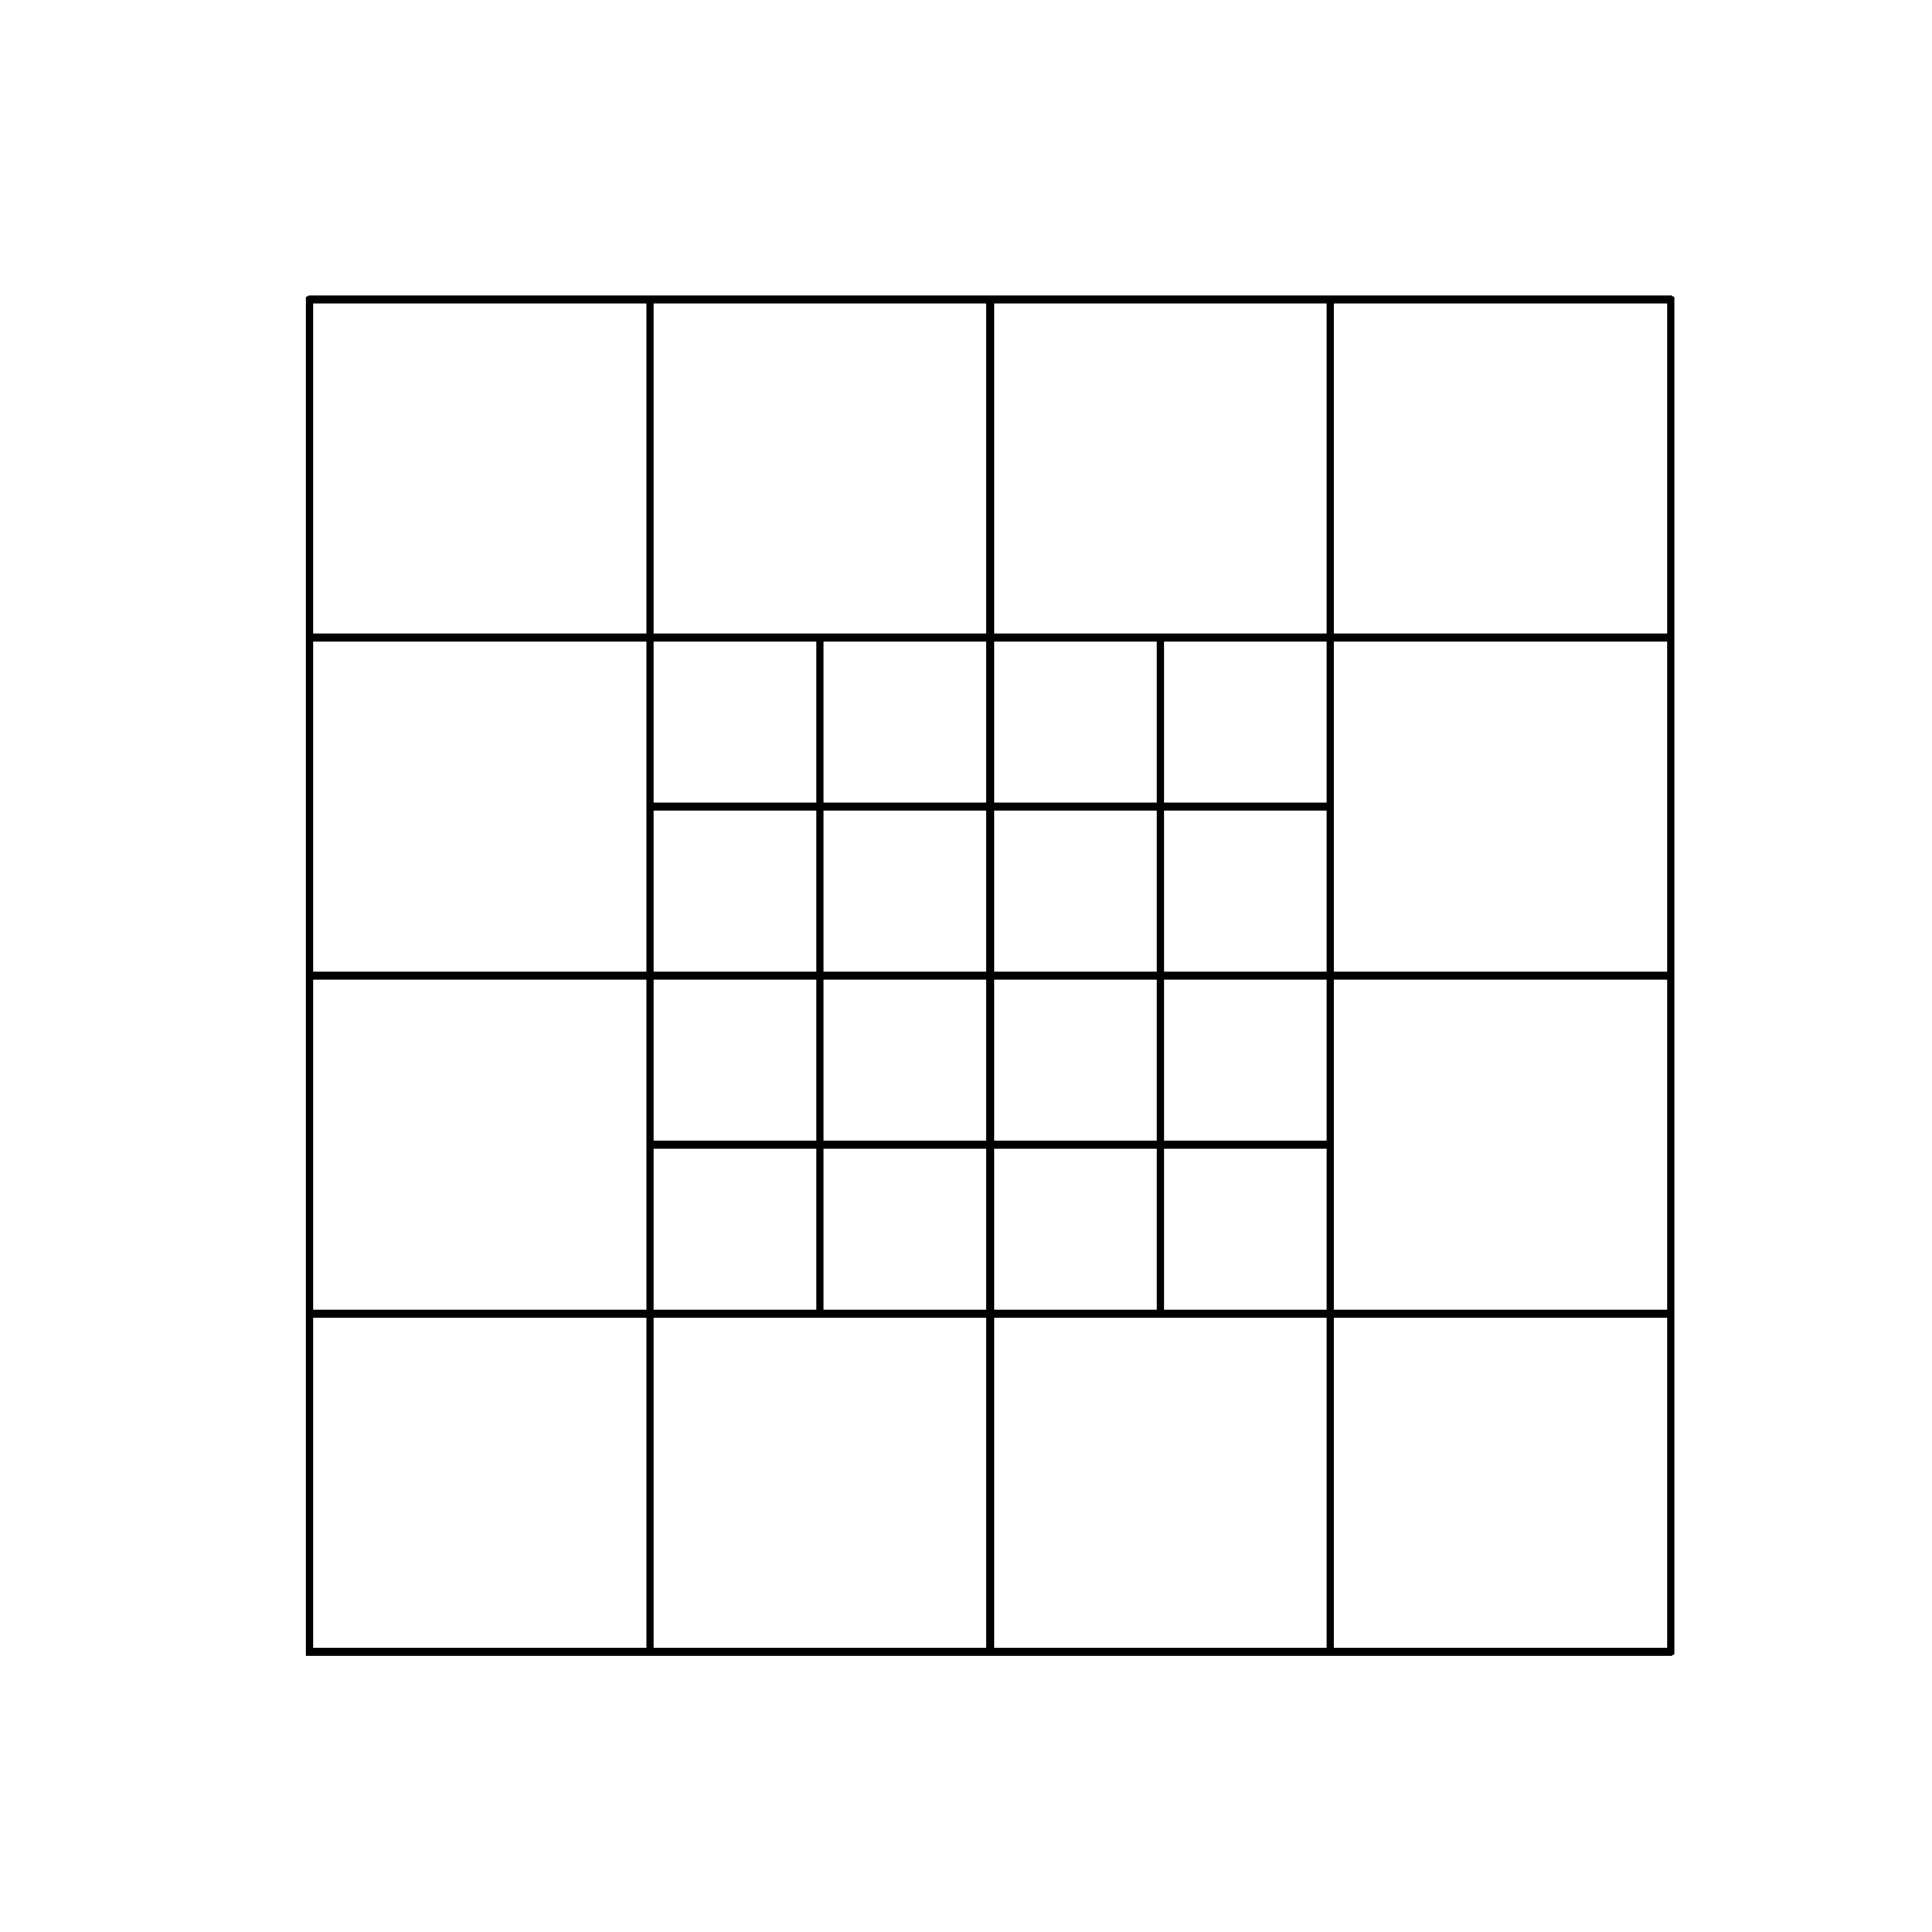
\includegraphics[width=0.95\linewidth, clip=true, trim={0 150 0 150}]{figures/adaptive-mesh-00.pdf}
        \caption{Initial mesh}
        \label{fig:adaptive-mesh-rebuild-00}
    \end{subfigure}
    \begin{subfigure}[t]{0.55\textwidth}
        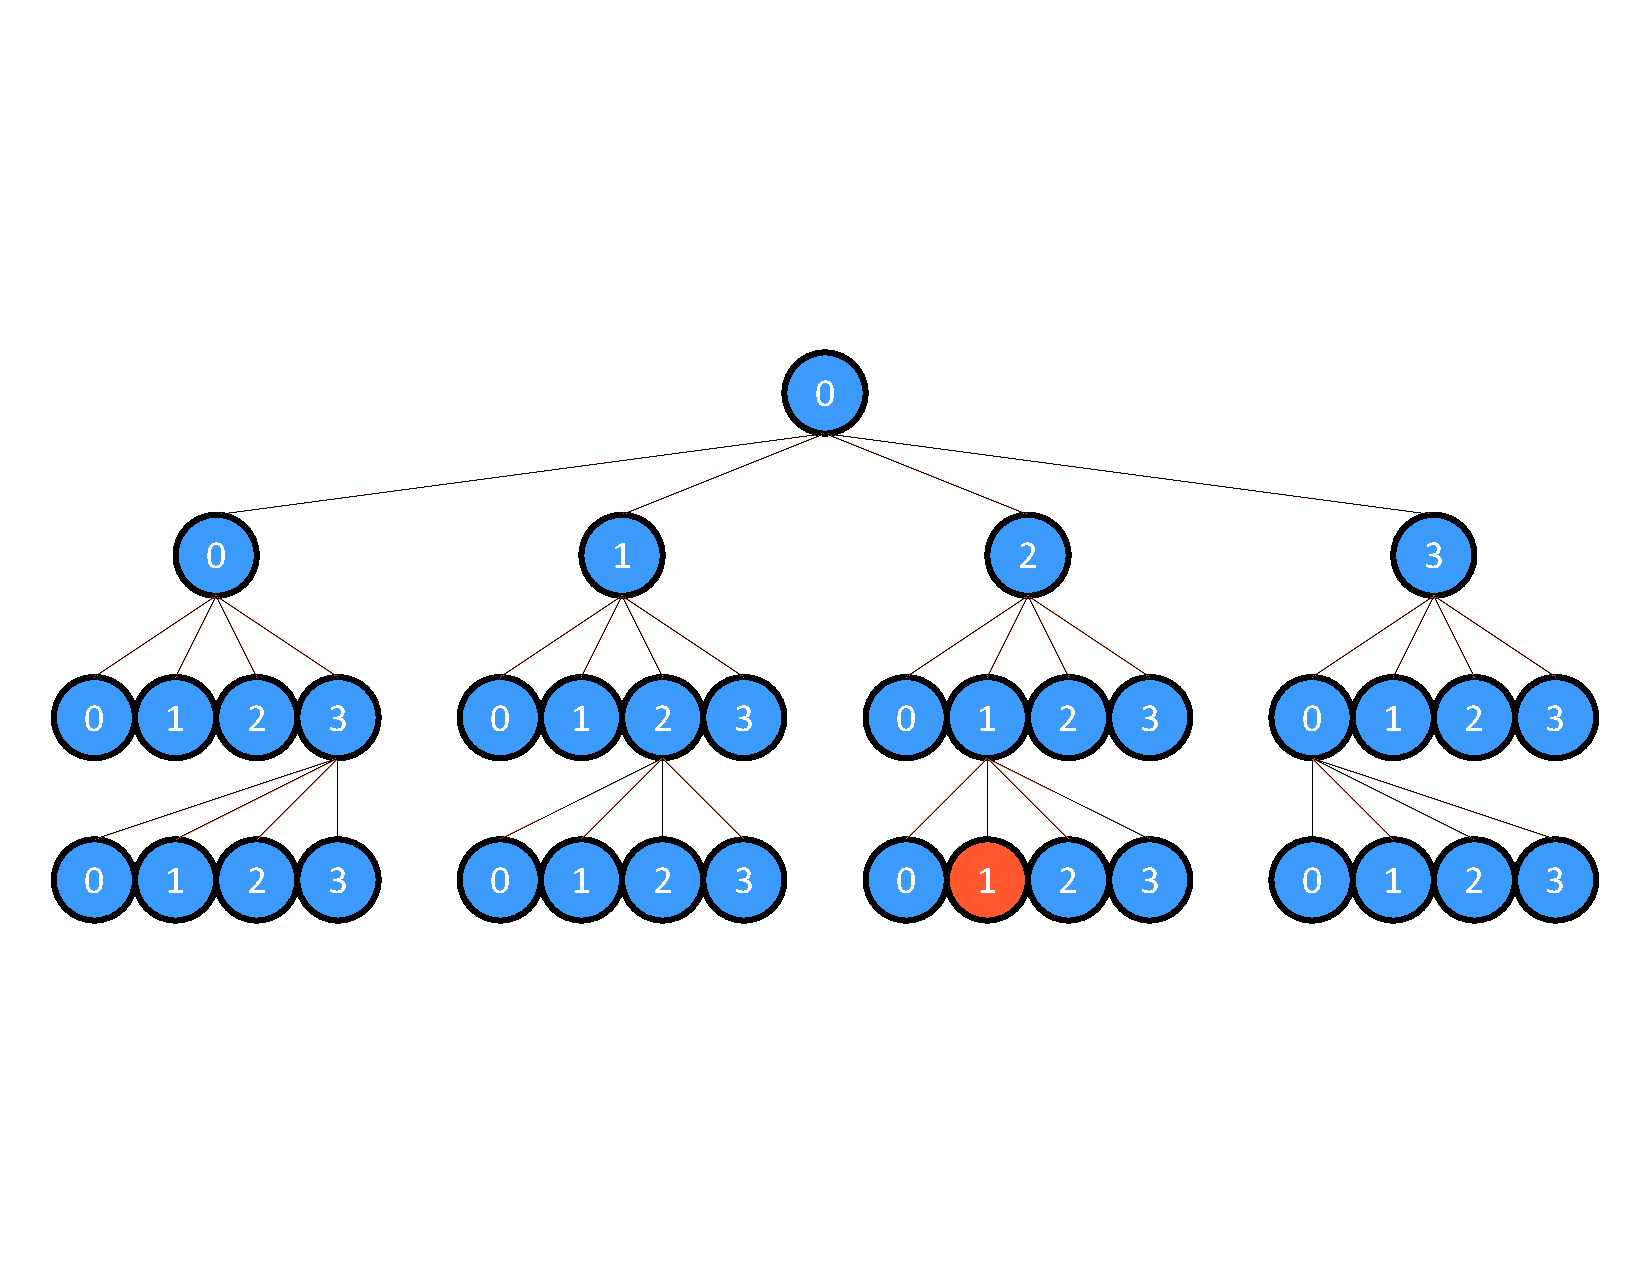
\includegraphics[width=0.95\linewidth, clip=true, trim={0 150 0 150}]{figures/adaptive-tree-rebuild-00.pdf}
        \caption{Initial quadtree}
        \label{fig:adaptive-tree-rebuild-00}
    \end{subfigure}
    \begin{subfigure}[t]{0.35\textwidth}
        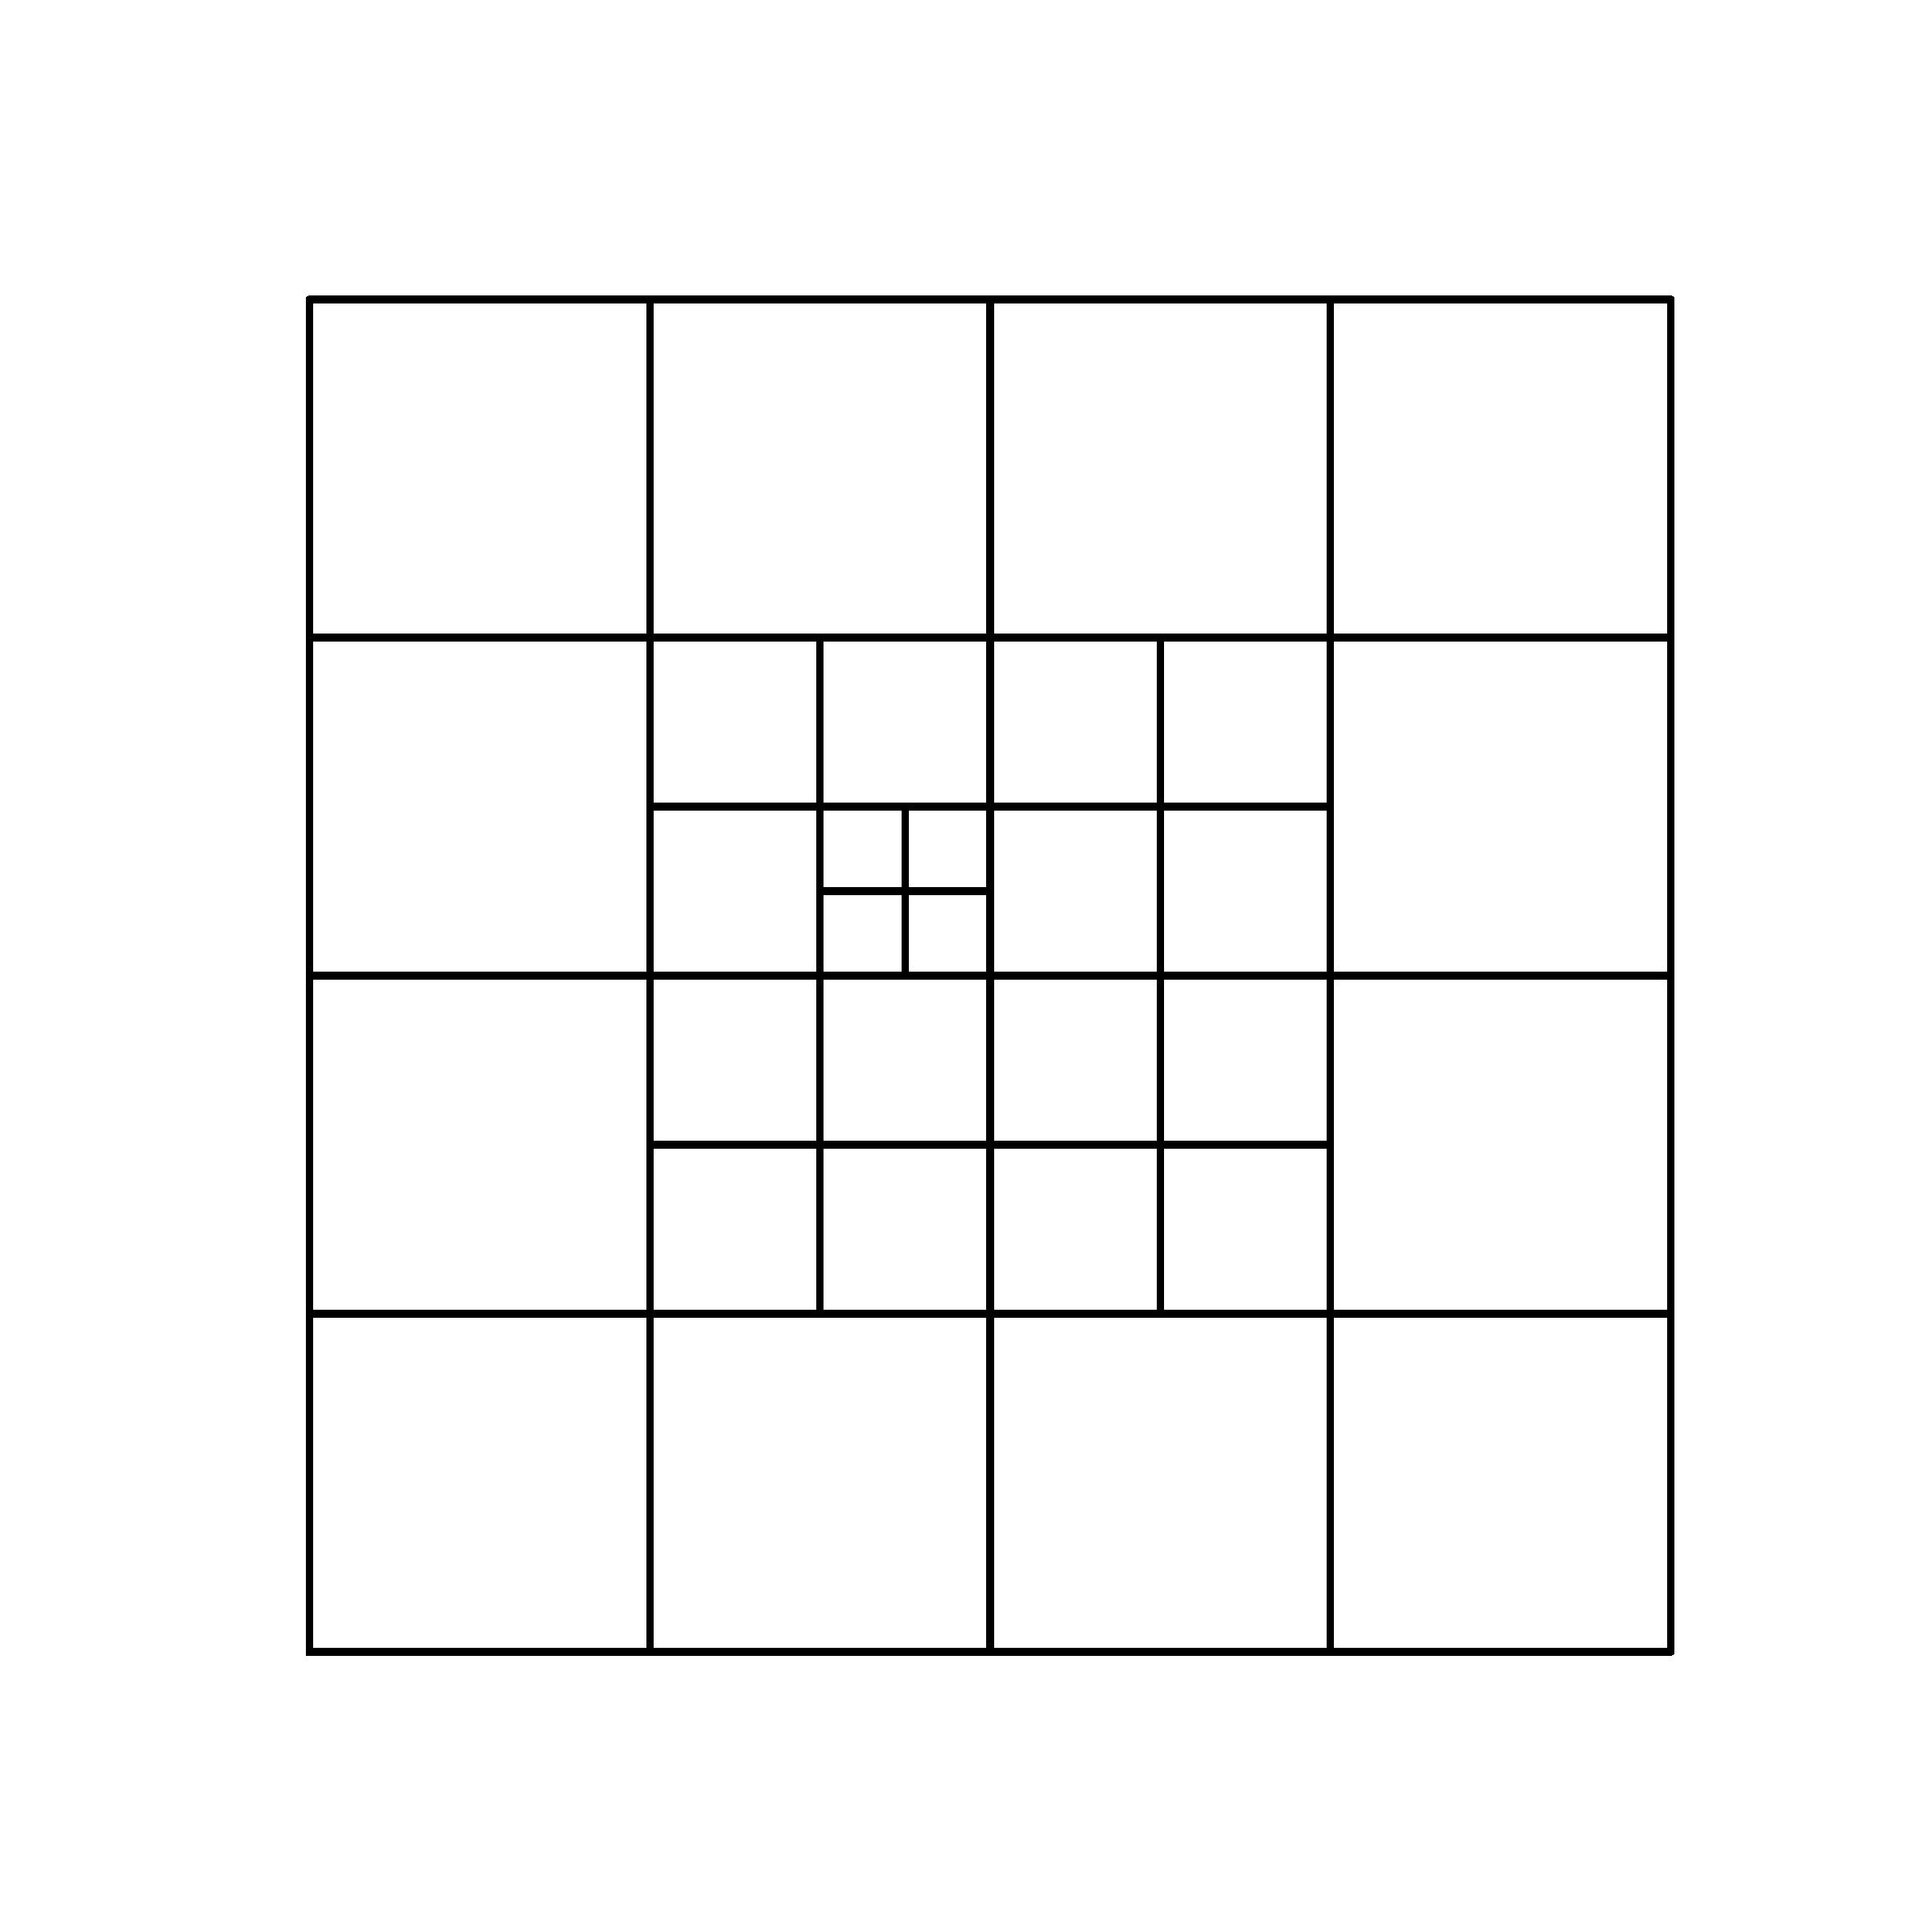
\includegraphics[width=0.95\linewidth, clip=true, trim={0 150 0 150}]{figures/adaptive-mesh-01.pdf}
        \caption{Refined mesh}
        \label{fig:adaptive-mesh-rebuild-01}
    \end{subfigure}
    \begin{subfigure}[t]{0.55\textwidth}
        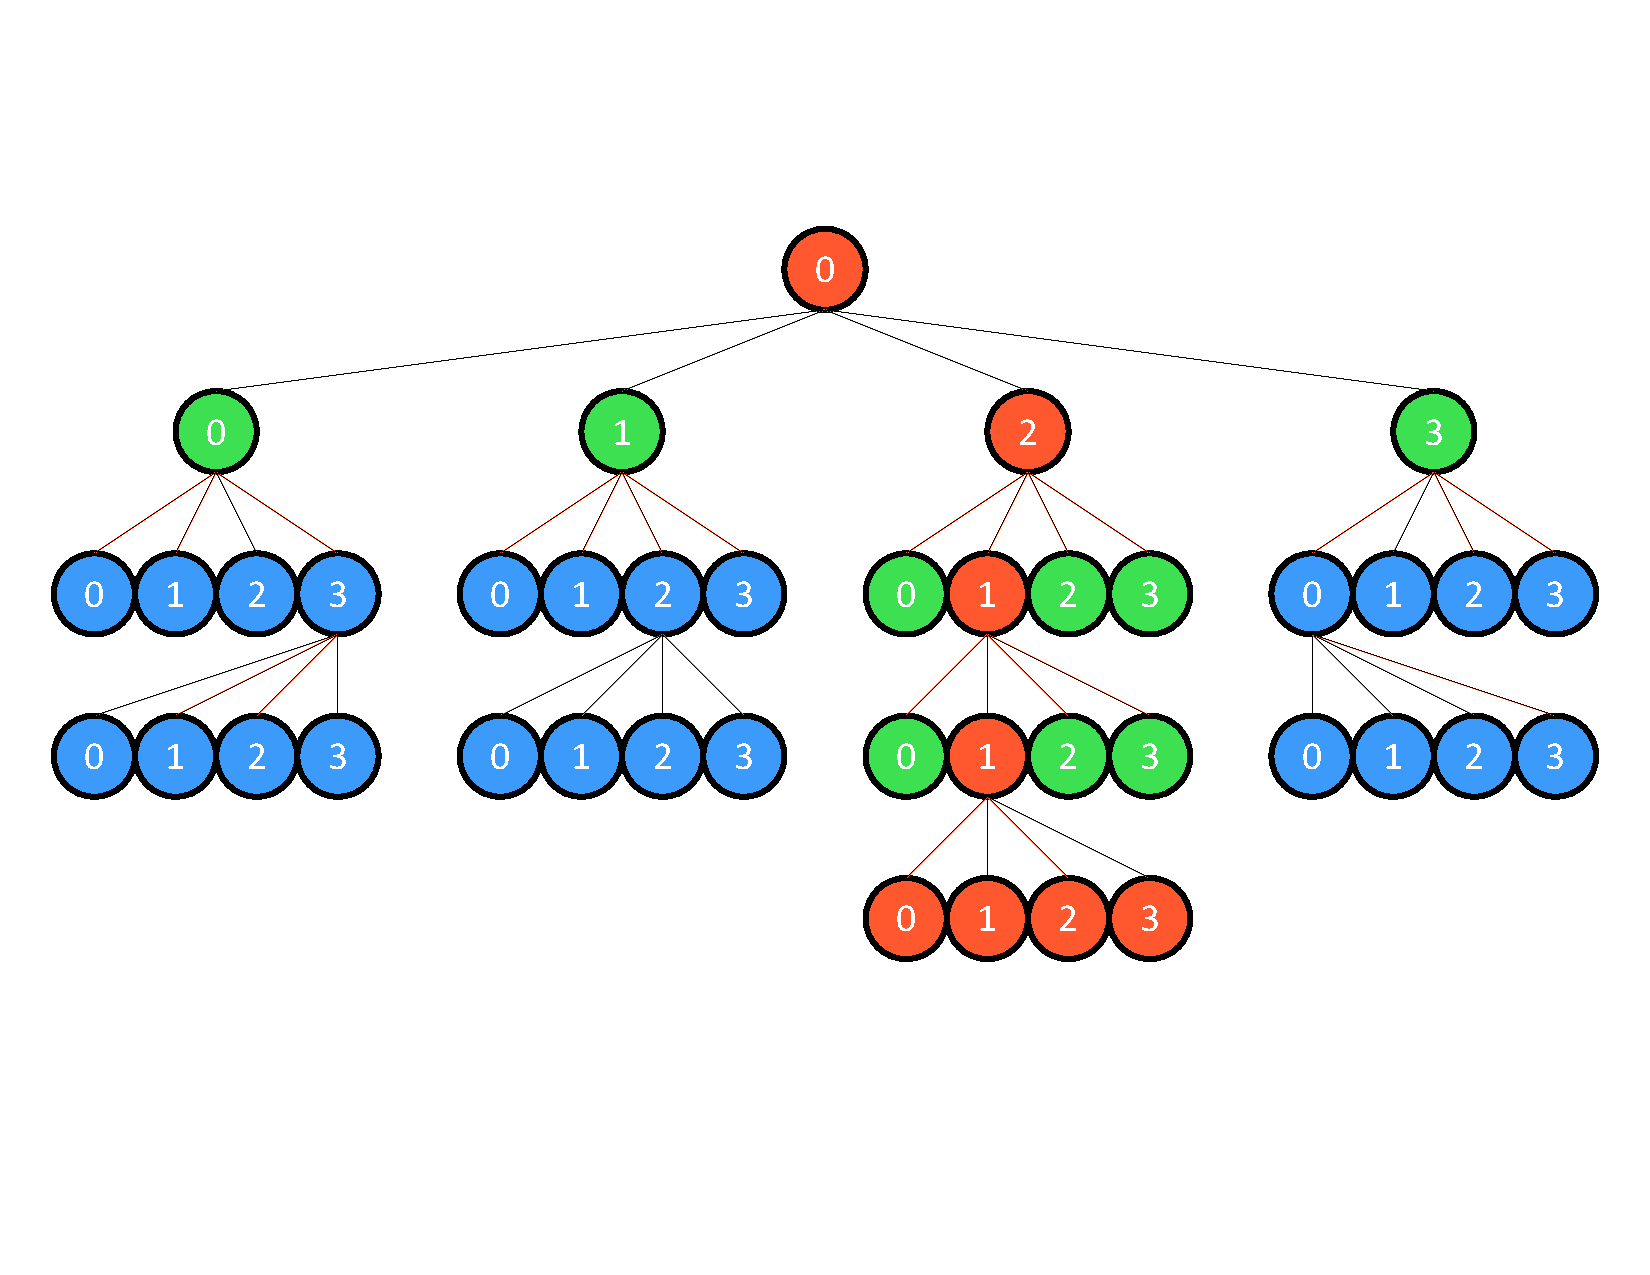
\includegraphics[width=0.95\linewidth, clip=true, trim={0 140 0 100}]{figures/adaptive-tree-rebuild-01.pdf}
        \caption{Refined quadtree}
        \label{fig:adaptive-tree-rebuild-01}
    \end{subfigure}
    \caption{Refining a mesh and a path-indexed quadtree. In (b), the red node is tagged for refinement. In (d), the red nodes are nodes where the factorization is either computed (for leaf nodes) or recomputed (for intermediate nodes). The green nodes indicate the dependencies of the red nodes within families; the operators on green nodes are used but not recomputed.}
    \label{fig:adaptive-mesh-rebuild}
\end{figure}

To motivate the derivation of such a technique, consider the two meshes and associated path-indexed quadtrees in \reffig{fig:adaptive-mesh-rebuild}. Suppose the domain-centered mesh in \reffig{fig:adaptive-mesh-rebuild-00} is refined an additional level, starting with the leaf-node indicated in \reffig{fig:adaptive-tree-rebuild-00}. The additional nodes are created and stored in the quadtree, which is reflected in \reffig{fig:adaptive-mesh-rebuild-01} and \reffig{fig:adaptive-tree-rebuild-01}. The question we seek to answer is this: how is the factorization set $\mathcal{S}$ affected by this change?

In each of the leaf nodes, the \gls{d2n} matrix \Ttau can be computed according to \refeqn{eq:Ttau-leaf} and the solution matrix \Stau can be formed. Recall, however, that at the leaf-level we do not form \Stau explicitly, rather we wrap fast solvers at the leaf-level that perform the action of \Stau. Similarly for the inhomogeneous data, we can form \htau according to \refeqn{eq:htau-leaf}.

Continuing up the tree, the newly formed leaf nodes can be merged to form \Ttau according to \refeqn{eq:Ttau-merged}, \Stau according to \refeqn{eq:Stau-merged}, \htau according to \refeqn{eq:htau-merged}, and \wtau according to \refeqn{eq:wtau-merged}. This accounts for the newly refined nodes and the original node that was tagged for refinement. However, the solution operators from each ancestor of the tagged node depend on the data from their respective children. Or, alternatively, a change in the solution operator set from a node affects each of ancestors' solution operators. So the 4-to-1 merge algorithm would need to be performed again for each respective parent up to the top of the quadtree.

For this example, the red nodes in \reffig{fig:adaptive-tree-rebuild-01} indicate the nodes that must be updated in the solution operator set $\mathcal{S}$. Note that these nodes are either the newly formed leaf nodes, the tagged node itself, or the direct ancestors of the tagged node. The green nodes indicate nodes whose data is necessary for the red nodes during the 4-to-1 merge, but does not need to be recomputed due to the refinement.

To further motivate the derivation of a direct method that can adapt its factorization, consider the amount of work necessary for the updated factorization set. The 4-to-1 merge would need to be performed once for each level in the tree. Compare this to the amount of work necessary to recompute the entire factorization set to reflect the updated mesh; the 4-to-1 merge would need to be performed for {\em all} families in the tree.

The rest of this chapter will outline the adaptive rebuild technique for the \gls{qahps} method. This will include the algorithm and implementation details with \pforest, convergence analysis comparing the full build and the adaptive rebuild, and a time comparison for both methods solving a Poisson equation.